\documentclass{article}
\PassOptionsToPackage{sort,numbers,square}{natbib}

\usepackage{nips_2018}
\usepackage[utf8]{inputenc} % allow utf-8 input
\usepackage[T1]{fontenc}    % use 8-bit T1 fonts
\usepackage{hyperref}       % hyperlinks
\usepackage{url}            % simple URL typesetting
\usepackage{booktabs}       % professional-quality tables
\usepackage{amsfonts}       % blackboard math symbols
\usepackage{nicefrac}       % compact symbols for 1/2, etc.
\usepackage{microtype}      % microtypography

% For citations
\usepackage{natbib}

% For algorithms
\usepackage{algorithm}
\usepackage{algorithmic}
\usepackage{hyperref}

%\newcommand{\theHalgorithm}{\arabic{algorithm}}


\usepackage{graphicx}
\usepackage{subfigure} 
\graphicspath{{../working-paper/}}


%Arash
\usepackage{amsmath}
\usepackage{amssymb}
\usepackage{mathrsfs}
\DeclareMathOperator*{\argmin}{argmin}
\usepackage{siunitx}

\usepackage{mathtools}
\mathtoolsset{showonlyrefs}

\renewcommand*{\figureautorefname}{Figure}%
\renewcommand*{\tableautorefname}{Table}%
\renewcommand*{\sectionautorefname}{Section}%
\renewcommand*{\subsectionautorefname}{Section}%
\renewcommand*{\subsubsectionautorefname}{Section}%


\usepackage{xcolor}
\newcommand{\attn}[1]{\textcolor{red}{TODO: #1}}
\newcommand{\one}{\mathbf{1}}
\renewcommand{\algorithmiccomment}[1]{\hfill $\rhd$ #1}



\title{Modeling trend in temperature volatility using generalized LASSO}

\author{Arash Khodadadi\\
 Department of Statistics\\
 Indiana University\\
 Bloomington, IN 47408 \\
 \texttt{arakhoda@indiana.edu}
\And
  Daniel J.\ McDonald \\
 Department of Statistics\\
 Indiana University\\
 Bloomington, IN 47408 \\
 \texttt{dajmcdon@indiana.cmu.edu}}


\begin{document} 


\maketitle


\begin{abstract}
words, words,

\end{abstract}



\section{Introduction}

Nonparametric variance estimation for spatio-temporal data.

\subsection{Motivating applications}

There is a considerable interest in determining if there is an increasing trend in the climate variability \citep{hansen_perception_2012,huntingford_no_2013}. An increase in the temperature variability will increase the probability of extreme hot outliers. It might be harder for the society to adapt to these extremes than to the gradual increase in the mean temperature \citep{huntingford_no_2013}.

In this project, we consider the problem of detecting the trend in the temperature volatility. All analyses are performed on a sub-set of the European Centre for Medium-Range Weather Forecasts (ECMWF) ERA-40 dataset \citep{uppala_era-40_2005}. This dataset include the temperature measurements over a grid over the earth from 1957 to 2002.~\citep{VasseurDeLong2014,TrenberthZhang2014,StatenKahn2016,Screen2014,FischerBeyerle2013}

Research on analyzing the trend in the volatility of spatio-temporal data is scarce. \citep{hansen_perception_2012} studied the change in the standard deviation (SD) of the surface temperature in the NASA Goddard Institute for Space Studies gridded temperature data set. In their analysis, for each geographical position, the mean of the temperature computed for the period 1951-1980 (called the base-period) at that position, is subtracted from the corresponding time series. Each time series is then divided by the standard deviation computed at each position and during the same time period. The distribution of the resulting data is then plotted for different periods. These distributions represent the deviation of the temperature for a specific period, from the mean in the base period, in units of the standard deviation in that period. The results showed that these distributions are widen for the resent time periods compared to 1951-1980.  \citep{huntingford_no_2013} took a similar approach in analysing the ERA-40 data set. However, in addition to the aforementioned method, they computed the distribution of the SDs in an alternative way: for each position and each time period, the deviation of the time-series at that position from the mean in that time period at that position was computed, and then divided by the SD of that position in the period before 1981. The results showed that there still is an increase in the SDs from 1958-1970 to 1991-2001, but this is much less than what is obtained from the method used in \citep{hansen_perception_2012}. The authors also computed the time-evolving global SD from the de-trended time-series at each position. The resulting curve suggested that the global SD has been stable.

These previous work (and other related research, e.g., \citep{rhines_frequent_2013}) have several shortcomings. First, no statistical analysis has been performed to examine if the change in the SD is statistically significant. Second, the methodologies for computing the SDs are rather arbitrary. The deviation of each time-series in a given period, is computed from either the mean of a base-period (as in \citep{hansen_perception_2012}), or from the given period (as in \citep{rhines_frequent_2013,huntingford_no_2013}). These deviations are then normalized using the SD of the base-period or the given period. No justification is provided for these choices. Third, the correlation between the observations is ignored. The observations in subsequent days and close geographical positions could be highly correlated. Without considering these correlations, any conclusion based on the averaged data could be flawed.

The main contribution of this work is to develop a new methodology for detecting the trend in the volatility of spatio-temporal data. In this methodology, the variance at each position and time, is considered as a hidden (un-observed) variable. The value of these hidden variables are then estimated by maximizing the likelihood of the observed data. We show that this formulation per se, is not appropriate for detecting the trend. To overcome this issue, we penalize the differences between the estimated variances of the observations which are temporally and/or spatially close to each other. This will result in an optimization problem called the \textit{generalized LASSO problem} \citep{tibshirani_solution_2011}. As we will see, the dimension of this optimization problem is very high and so the standard methods for solving the generalized LASSO cannot be applied directly. We investigate two methods for solving this optimization problem. In the first method, we adopt an optimization technique called alternative direction method of multipliers (ADMM) \citep{boyd_distributed_2011}, to divide the total problem into several sub-problems of much lower dimension and show how the total problem can be solved by iteratively solving these sub-problems. The second method, called the \textit{linearized ADMM algorithm} \citep{parikh_proximal_2014} solves the main problem by iteratively solving a linearized version of it. We will compare the benefits of each method.

Also neuroscience.


\subsection{Related work}

Mention ~\citep{KimKoh2009,HallacPark2017}. Also, ~\citep{Tibshirani2014,TibshiraniTaylor2011}. Find Sharpnack Tibshirani. ARCH/GARCH.

\citep{SadhanalaWang2017,LinSharpnack2017,WangSharpnack2016}~\citep{RamdasTibshirani2016}

\subsection{Main contributions}

\section{$\ell_1$-trend filtering for estimating variance of a time-series}

$\ell_1$-trend filtering was proposed by \citep{kim_$ell_1$_2009} as a method for estimating a smooth, time-varying trend. It is formulated as the optimization problem
% : a time-series $y_t$, $t=1,...,T$ is observed and we believe that it consists of a smooth trend and a stochastic component and the goal is to estimate the trend. The estimated trend is desired to be smooth, but at the same time, we seek small estimated residuals (stochastic component). These two objectives cannot be achieved simultaneously and so a trade-off between them should be made. In $\ell_1$-trend filtering, this trade-off is formulated as the following convex optimization problem:
\begin{equation}
\min_{\beta} \frac{1}{2} \sum_{t=1}^{T} (y_t-\beta_t)^2+\lambda \sum_{t=1}^{T-2} |\beta_t-2\beta_{t+1}+\beta_{t+2}|
\end{equation}
or equivalently:
\begin{equation}
\min_{\beta} \frac{1}{2} \lVert y-\beta \lVert_2^2+\lambda \lVert D\beta\lVert_1
\label{eq:l1tf}
\end{equation}
 where $y_t$ is an observed time-series, $\beta$ is the smooth trend, $D$ is a $T-2\times T$ matrix, and $\lambda$ is a tuning parameter which balances fidelity to the data (small errors in the first term) with a desire for smoothness. 
% The \textit{penalty matrix} is:
% \begin{equation}
% D=\begin{bmatrix}
% 1 & -2 & 1 &  &  &  &\\ 
% & 1 & -2 & 1 &  &  &\\ 
% &  & \ddots & \ddots & \ddots  &  &\\ 
% &  & & 1 & -2 & 1 &  \\ 
% &  &  &   & 1 & -2 & 1 
% \end{bmatrix}
% \label{eq:d_matrix}
% \end{equation}
%The first term in \eqref{eq:l1tf} penalizes large residuals while the second term encourages smooth estimated $\beta$.
With the penalty matrix $D$, the estimated $\beta$ will be piecewise linear. \citep{kim_$ell_1$_2009} proposed a specialized primal-dual interior point (PDIP) algorithm for solving \eqref{eq:l1tf}. From a statistical perspective, \eqref{eq:l1tf} is a constrained maximum likelihood problem with independent observations from a normal distribution with common variance, $y_t \sim \mbox{N}(\beta_t, \sigma^2)$, subject to a piecewise linear constraint on $\beta$.

% The results of applying $\ell_1$-trend filtering on the Bloomington time-series are shown in \autoref{fig:bloom_detrended}. The left panel shows the original time-series (blue) together with the estimated $\beta$ (red) and the right panel shows the residuals $y_t-\beta_t$ (blue). As it can be seen, the estimated $\beta$s are piecewise linear. The number of linear segments is determined by the value of $\lambda$. Here, we chose $\lambda=500$. The choice of $\lambda$ is a model selection problem and we will return to it in the next section ???.

\subsection{Extension to variance estimation}
\label{sec:l1tf_var}


Inspired by the $\ell_1$-trend filtering algorithm, we propose a non-parametric model for estimating the variance of a time-series. To this end, we assume that at each time step $t$, there is a hidden variable $h_t$ such that conditioned on $h_t$ the observations $y_t$ are independent normal variables with zero mean and variance $\exp(h_t)$. The negative log-likelihood of the observed data in this model is $l(y|h) \propto -\sum_{t=1}^Th_t - y_t^2e^{-h_t}$. Crucially, we assume that the hidden variables $h_t$ vary smoothly. To impose this assumption, we estimate $h_t$ by solving the penalized, negative log-likelihood:
\begin{equation}
\min_h -l(y|h)+\lambda \lVert Dh \lVert_1
\label{eq:l1tf_var}
\end{equation}
 where $D$ has the same structure as above.

\attn{explain the objective more. give the AR(1) example. Explain what you loses by this assumption (ACF,forecasting). Also explain that the covariace matrix is diagonal so it cannot capture the covariance structure. But incontrast to spatial stat literature, it does not make any assumption on estimated variances. Compare to Hallac et al and Lingren et al.}

As with~\eqref{eq:l1tf}, one can solve~\eqref{eq:l1tf_var} using the PDIP algorithm (as in, e.g., \texttt{cvxopt}~\citep{andersen_cvxopt:_2013}). First, we note that this is a generalized LASSO problem \citep{tibshirani_solution_2011}. The dual of a generalized LASSO with the objective $f(x)+\lambda \lVert Dx \lVert_1$ is: 
\begin{align}
\min_\nu&\quad f^*(-D^\top\nu) \\
\mbox{s.t.}&\quad \lVert \nu \lVert_\infty \le \lambda
\end{align}
 where $f^*(\cdot)$ is the Fenchel conjugate of $f$: $f^*(u)=\max_x u^tx-f(x)$. It is simple to show that 
\begin{equation}
f^*(\mathsf{u})=\sum_t (u_t-1)\log\frac{y_t^2}{1-u_t} + u_t-1.
\label{eq:conj}
\end{equation}
Writing
\[
  r_w(v,\mu_1,\mu_2):=
  \begin{bmatrix}
    \nabla f^*(-D^\top v) + D(v-\lambda \one)^\top \mu_1 -
    D(v+\lambda \one)^\top \mu_2\\
    -\mu_1(v-\lambda\one)+\mu_2(v + \lambda\one) -w^{-1}\one
  \end{bmatrix}
  =
  \begin{bmatrix}
  0\\0\end{bmatrix}
\]
for $w>0$, where $\mu_1$ and $\mu_2$ are dual variables for the $\ell_\infty$ constraint in the dual problem. As $w\rightarrow\infty$, the solution to this nonlinear system reduces to the KKT conditions. Therefore, the PDIP method takes Newton steps to solve the system for a series of increasing values of $w$. \autoref{alg:pdip} provides the details.
\begin{algorithm}
  \caption{PDIP for $\ell_1$ variance estimation}
  \label{alg:pdip}
  \begin{algorithmic}
    \REQUIRE $\lambda>0$, $w>0$, $\nu\leftarrow 0$, $\mu_1\leftarrow 0$, $\mu_2\leftarrow 0$, $J\in\mathbb{Z}^+$, $\{w_k\}$ \COMMENT{Initialization}
    \FOR[Central path]{$k=1,2,\ldots$}
    \FOR[Newton updates]{$j=1,\ldots,J$}
    \STATE Solve $A [\Delta\nu\; \Delta\mu_1\; \Delta\mu_2]^\top=r^j_{w_k}$ to find the search direction.
    \STATE $\quad\quad A$ is the Jacobian of $r_w$.
    \STATE Update $r^{j+1} \leftarrow r^j + [\Delta\nu\; \Delta\mu_1\; \Delta\mu_2]^\top$.
    \ENDFOR
   \ENDFOR
   \RETURN $h=-D^\top\nu$ \attn{Is this right??}
  \end{algorithmic}
\end{algorithm}


\subsection{Extension to spatio-temporal data}
\label{sec:exten}

The method in the previous section can be used to estimate the variance of a single time-series. In this section, we extend this method to the estimation of the variance of spatio-temporal data.

At a specific time $t$, the data is measured on a grid of points with $n_r$ rows and $n_c$ columns. Let $y_{ijt}$ denote the value of the observation at time $t$ on the $i^\text{th}$ row and $j^\text{th}$ column of the grid, and $h_{ijt}$ denote the corresponding hidden variable. We seek to impose both temporal and spatial smoothness constraints on the hidden variables. Specifically, we seek a solution for $h$ which is piecewise linear in time and piecewise constant in space \footnote{The assumption that the variance is spatially piecewise constant simplifies the computations. The justification for this assumption is that we are interested in examining the trend in the variance over time and not over space.}. This can be achieved by solving the following optimization problem:

\begin{equation}
\begin{aligned}
\min_h &\sum_{i,j,t}h_{ijt}+y_{ijt}^2e^{-h_{ijt}}\\
&+\lambda_t \sum_{i,j} \sum_{t=1}^{T-2} \big|h_{ijt}-2h_{ij(t+1)}+h_{ij(t+2)}\big|\\
&+\lambda_s \sum_{t,j} \sum_{i=1}^{n_r-1} \big|h_{ijt}-h_{(i+1)jt}\big|\\
&+\lambda_s \sum_{t,i} \sum_{j=1}^{n_c-1} \big|h_{ijt}-h_{i(j+1)t}\big|
\end{aligned}
\label{eq:l1tf_var_st}
\end{equation}

The first term in the objective is the negative log-likelihood (minus a constant term). The second term is the temporal penalty for the time-series at each location $(i,j)$. The third and fourth terms, penalize the difference between the estimated variance of two vertically and horizontally adjacent points, respectively. This penalty is a special case of the penalty used in the \textit{trend filtering on graphs }\citep{wang_trend_2016} (where the difference between the estimated values of the signal at each two nodes connected with an edge is penalized.). The optimization problem \eqref{eq:l1tf_var_st} can be written in the matrix form. Let $h$ be a vector whose first $T$ entries are $h_{11t}$ for $t=1,...,T$, its next $T$ entries are $h_{21t}$ and so on. Then the optimization problem in the matrix form is as follows:

\begin{equation}
\min_h -l(y|h)+ \Lambda^t \lVert D_{total}h \lVert_1
\label{eq:l1tf_var_st_mat}
\end{equation}

Let, $\textbf{e}_n$ denote a vector of size $n$ with all entries being equal to 1. We have: $\Lambda^t=(\lambda_t\textbf{e}_{n_t}^t|\lambda_s\textbf{e}_{n_s}^t)$, $D_{total}^t=[D_{t}^t|D_{s}^t]$, where $n_t$ and $n_s$ are the number of rows of $D_{t}$ and $D_{s}$, respectively (see below). The matrix $D_t$ is the following block-diagonal matrix and corresponds to the temporal penalty:

\begin{equation}
D_t=\begin{bmatrix}
D &  & \\ 
 & \ddots & \\
 &  & D
\end{bmatrix}
\label{eq:d_t_matrix}
\end{equation}

 where $D$ was defined in \eqref{eq:d_matrix}. The number of the diagonal blocks is equal to the grid size $n_r \times n_c$. Each row of the matrix $D_s$ corresponds to one spatial constraint in \eqref{eq:l1tf_var_st}. For example, the first $T$ rows correspond to $|h_{11t}-h_{21t}|$ for $t=1,...,T$, the next $T$ rows correspond to $|h_{11t}-h_{12t}|$, and so on.

\attn{Detailed discussion of the PDIP to here}

The dual of this problem is:

\begin{equation}
\begin{aligned}
\min_\nu f^*(-D_{total}^t\mathsf{\nu}) \\
s.t. \,\,\, | \nu_i | \le \Lambda_i
\end{aligned}
\label{eq:dual}
\end{equation}

 where $f^*$ is given in \eqref{eq:conj}.


\section{Optimization}
For a spatial grid of size $n_r \times n_c$ and for $T$ time steps, we have $n_t=3n_rn_c-Tn_c-2n_rn_c$ and $n_s=n_rn_cT$. For a grid over the united states and for weekly averaged data of 10 years we have $n_r=32$, $n_c=68$, $T=521$ and so $n_t\approx 3.5\times10^6$ and $n_s \approx 1.0\times10^6$. Therefore, the size of the optimization problem \eqref{eq:dual} is about $n_t\approx 4.5\times10^6$. In each step of the PDIP algorithm, we need to solve a linear system of equations in the form $z=Ax$ where $A$ is a square matrix of size $2(n_t+n_s)$ (see \citep{boyd_convex_2004} equation 11.54). Therefore, applying the PDIP directly for solving the optimization problem \eqref{eq:dual} is infeasible.

In the next section, we develop an ADMM algorithm for solving this problem. The idea is to cast the problem \eqref{eq:dual} as a so-called \textit{consensus optimization problem} \citep{boyd_distributed_2011} and solve it by breaking the problem into smaller sub-problems using an ADMM-based algorithm. Next, we first give a brief overview of the consensus optimization problem and then explain how the problem \eqref{eq:l1tf_var_st_mat} can be solved in this framework.

\subsection{Consensus optimization}
\label{sec:consOpt}

A general form consensus optimization problem is in the form $\min_z \sum_i f_i(z)$, $z\in\mathbb{R}^n$. We can define a set of \textit{local variables} $x_i\in \mathbb{R}^{n_i}$ such that $\sum_i f_i(z)=\sum_i f_i(x_i)$. We follow the notation of \citep{boyd_distributed_2011} closely. Let $k=\mathscr{G}(i,j)$ which means that the $j^\text{th}$ entry of $x_i$ is $z_k$ (or $(x_i)_j=z_k$) and define $\tilde{z}_i \in \mathbb{R}^{n_i}$ by $(\tilde{z}_i)_j=(x_i)_j$. Then the original unconstrained optimization problem is equivalent to the following constrained optimization problem:

\begin{equation}
\begin{aligned}
\min_{\{x_1,...,x_N  \}} \sum_i f_i(x_i)\\
 s.t. \,\,\, \tilde{z}_i=x_i \,\,\,\,\,\,
\end{aligned}
\end{equation}

Now, we can apply ADMM to the \textit{augmented Lagrangian} of this problem. This results in the following ADMM updating steps at each iteration $m$:

\begin{equation}
\begin{aligned}
& x_i^{m+1}:=\argmin_{x_i} \bigg( f_i(x_i) + (u_i^m)^t x_i + (\rho/2) \lVert x_i-\tilde{z}_i^m \lVert_2^2\bigg)\\
& z_k^{m+1}:=(1/S_k)\sum_{\mathscr{G}(i,j)=k} (x_i^{m+1})_j\\
& u_i^{m+1}:=u_i^m + \rho (x_i^{m+1}-\tilde{z}_i^{m+1})
\end{aligned}
\label{eq:ADMM_steps}
\end{equation}

Here, $S_k$ is the number of local variable entries that correspond to $z_k$, and $u_i$ are the Lagrange multipliers. 

To solve the optimization problem \eqref{eq:l1tf_var_st_mat} or \eqref{eq:l1tf_var_st} using the method explained in the previous section we need to two address two questions: first, how to choose the local variables $x_i$, and second, how to solve the optimization problem for updating these variables (the first line of \eqref{eq:ADMM_steps}). 

Obviously, the global variable in the problem \eqref{eq:l1tf_var_st} is $z=h$. The global variable can be index by the spatial coordinate and the temporal step. In \autoref{fig:data_cube}, $z$ is represented as a cube. We can decompose $z$ into sub-cubes. An example of this decomposition is shown in the figure by white lines. It is easy to see that with this definition of $x_i$, the objective \eqref{eq:l1tf_var_st_mat} decomposes as $\sum_i f_i(x_i)$ where $f_i(x_i)=-l(y_i|x_i)+\lVert \Lambda_i^t D_ix_i \lVert_1$. 

%TODO: re-write this part. it is very confusing.

\begin{figure}[tb]
	\vskip 0.2in
	\begin{center}
		\centerline{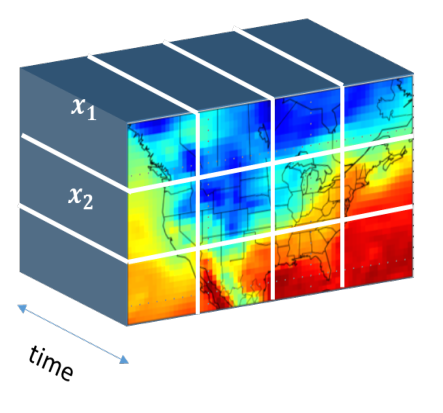
\includegraphics[width=.5\columnwidth]{Figures/data_cube}}
		\caption{The cube represents the global variable $z$ in space and time. The sub-cubes specified by the white lines are $x_i$.}
		\label{fig:data_cube}
	\end{center}
	\vskip -0.2in
\end{figure} 

By this definition of $x_i$, the update step for $x_i$ is the following optimization problem: $x_i^{m+1}:=\argmin_{x_i} ( f_i(x_i) + (u_i^m)^t x_i + (\rho/2) \lVert x_i-\tilde{z}_i^m \lVert_2^2)$.

\attn{Redo the below and move to the section on PDIP above}

We solve this using the PDIP method. To this end we first need to compute the dual of the problem. It can be shown that the dual of this problem is:

%TODO: write the appendix

\begin{equation}
\begin{aligned}
\min_\nu f_i^*(-D_i^t\nu_i) \\
s.t. \,\,\, | (\nu_i)_j | \le (\Lambda_i)_j
\end{aligned}
\label{eq:dual_x_update}
\end{equation}

 where:

\begin{equation}
\begin{aligned}
f^*_i(q)&=\sum_j (q_i)_j (w_i)_j -(w_i)_j-(y_i)_j^2 e^{-(w_i)_j} - \\
& (\rho/2)((w_i)_j-(\alpha_i^m)_j)^2\\
&\alpha_i^m =\hat{z}_i^m-u_i^m\\
(w_i)_j&=\mathscr{W}\bigg(\frac{(y_i)_j^2}{\rho}\exp\bigg[\frac{1-q_j-\rho(\alpha_i^m)_j}{\rho}\bigg]\bigg)-\\
& \frac{1-q_j-\rho(\alpha_i^m)_j}{\rho}
\end{aligned}
\label{eq:conj_x_update}
\end{equation}

In these equations, $\mathscr{W}$ is the \textit{Lambert function} \citep{corless_lambertw_1996}. To use the PDIP method, we also need to compute the gradient and Hessian of $f_i^*(-D_i^t\nu_i)$. This involves computing the derivatives of the Lambert functions. The primal solution $x_i$ can be obtained from the dual solution $\nu_i$ in \eqref{eq:dual_x_update} by setting $x_i=w_i$ where $w_i$ is defined in the last equation of \eqref{eq:conj_x_update}. 

The complete ADMM algorithm for estimating the variances is represented in \autoref{alg:ADMM}. All the computations in the three updating steps \eqref{eq:ADMM_steps} can be performed in parallel. The number of rows and columns of the sub-cubes should be chosen so that the updating of $x_i$ could be performed in one processor. We choose $3\times3\times521$ sub-cubes.

\begin{algorithm}[tb]
	\caption{ADMM for sparse estimation of variance of spatio-temporal data}
	\label{alg:ADMM}
	\begin{algorithmic}
		\STATE {\bfseries Input:} data $y$, mapping $\mathscr{G}(i,j)$, $\rho,\lambda_t,\lambda_s$
		\STATE Initialization: $x_i^0=z^0=u_i^0=\textbf{0}$.
		\FOR{$m=1,2,...$ }
			\FOR{$i=1$ {\bfseries to} $N_{sub-cubes}$}
				\STATE compute $\nu_i$ from \eqref{eq:dual_x_update}
				\STATE compute $w_i$ from \eqref{eq:conj_x_update}
				\STATE set $x_i^m:=w_i$
			\ENDFOR
		\STATE Compute $z^m$ from  \eqref{eq:ADMM_steps}
		\STATE Compute $u_i^m$ from  \eqref{eq:ADMM_steps}
		\ENDFOR
	\end{algorithmic}
\end{algorithm}

This algorithm divides the main optimization problem into several sub-problems and in each iteration solves these sub-problems and then performs a consensus step to make the solutions of these sub-problems agree with each other. These sub-problems can be solved independently which makes this algorithm appealing for parallelization: in each iteration, each of these sub-problems can be sent into a separate computer and then all the solutions can be sent into a single computer which performs the consensus step. Therefore, in each iteration, the computation time will be equal to the time of solving each sub-problem plus the time of communicating the solutions to the master computer and then performing the consensus step. Since each sub-problem is small, with parallelization, the computation time in each iteration will be small. In addition, our experiments with several values of $\lambda_t$ and $\lambda_s$ showed that the algorithm converges in few hundreds iterations. Solving each sub-problem on a machine with four 3.20GHz Intel i5-3470 cores takes less than 3 seconds on average, and so for example if we assume that communication time is 10 seconds and the algorithm converges in 300 iterations, with parallelization on $N_{sub-cubes}$ machines, the algorithm will converge in about 1 hour. Assuming that we use $N_{sub-cubes}$ machines and that the convergence rate of the algorithm is independent of the grid size, this time will be independent of the grid size.

If we perform these computations on a single machine, the computation time grows linearly with $N_{sub-cubes}$. For example, for the data in a grid over the united states and using $3\times3\times521$ sub-cubes each iteration of the algorithm will take about 20 minutes on a single machine and so with 300 iterations it will take several days to converge. Given that we need to compute the solution for several values of the parameters $\lambda_t$ and $\lambda_s$, this computation time is not feasible.

Therefore, this algorithm is only useful if we can parallelize the computation over several machines. In the next section, we describe another algorithm which makes the computation feasible on a single machine.

\subsection{Linearized ADMM}
\label{sec:linADMM}

In this section, we describe \textit{Linearized ADMM algorithm} \citep{parikh_proximal_2014} which, as we will see, makes the computation on a single machine feasible.

Consider the following optimization problem:

\begin{equation}
\min_x f(x)+g(Dx)
\label{eq:linADMM_opt}
\end{equation} 

 where $x\in \mathbb{R}^n$ and $D\in \mathbb{R}^{m\times n}$. Each iteration of the linearized ADMM algorithm for solving this problem has the following form:

\begin{eqnarray}
\begin{aligned}
x^{k+1} & := \textbf{prox}_{\mu f} \big(x^k - (\mu/\rho)D^T (D x^k - z^k + u^k )\big)\\
z^{k+1} & := \textbf{prox}_{\rho g} \big(D x^k + u^k\big)\\
u^{k+1} & := u^k + D x^{k+1} - z^{k+1}
\end{aligned}
\label{eq:linADMM_steps}
\end{eqnarray}

 where $z,u\in \mathbb{R}^m$ and the \textit{proximal operator} is defined as follows:

\begin{equation}
 \textbf{prox}_{\alpha f}(u) = \min_x \,\, \alpha \cdot f(x)+\frac{1}{2} \lVert x-u \rVert^2
\label{eq:linADMM_prox}
\end{equation}

This algorithm belongs to the general class of \textit{proximal algorithms} for solving convex optimization problems. For more details about these algorithms see \citep{parikh_proximal_2014}. 

The optimization problem \eqref{eq:l1tf_var_st} can be put into the form \eqref{eq:linADMM_opt} as follows:

\begin{equation}
\begin{aligned}
& f(x):= \sum_{k} f_k(x_k) := \sum_{k}x_k+y_{k}^2e^{-x_{k}}\\
& g(z):= \sum_{l} g_l(z_l) := \sum_{l} \lambda_l |z_l|\\
& z= Dx
\end{aligned}
\label{eq:linADMM_fg}
\end{equation}

 where $y_k$ is the $k^{th}$ entry of the vector whose entries are $y_{ijt}$, and $\lambda_l$ is the $l^{th}$ entry of the vector $\Lambda^t=(\lambda_t\textbf{e}_{n_t}^t|\lambda_s\textbf{e}_{n_s}^t)$ (see \autoref{sec:exten}).

To perform the steps in \eqref{eq:linADMM_steps}, we need to evaluate $\textbf{prox}_{\mu f}$ and $\textbf{prox}_{\rho g}$. The proximal algorithms are feasible only if these proximal operators can be evaluated efficiently which, as we show next, is the case for our problem. 

Let $\big(\textbf{prox}_{\mu f}(u)\big)_k$ be the $k^{th}$ entry of $\textbf{prox}_{\mu f}(u)$. From the \textit{separable sum} property of the proximal operators we have (see \citep{parikh_proximal_2014}, section 2.1):

\attn{Make this a theorem}

\begin{equation}
\bigg(\textbf{prox}_{\mu f}(u)\bigg)_k = \textbf{prox}_{\mu f_k}(u_k)\\
\label{eq:linADMM_sepSum}
\end{equation}

Similarly, evaluating $\textbf{prox}_{\rho g}$ reduces to evaluating the proximal operators of scalar functions. We have:

\begin{equation}
\textbf{prox}_{\mu f_k}(u_k)=\min_{x_k} \,\, \mu\big(x_k+y_{k}^2e^{-x_{k}}\big)+\frac{1}{2}  (x_k-u_k)^2\\
\label{eq:linADMM_proxf}
\end{equation}

By setting the derivative with respect to $x_k$ of the function to zero we obtain:

\begin{equation}
\textbf{prox}_{\mu f_k}(u_k)=\mathscr{W}\bigg(\frac{y_k^2}{\mu} \exp\bigg(\frac{1-\mu u_k}{\mu}\bigg) \bigg) + \frac{1-\mu u_k}{\mu}\\
\label{eq:linADMM_proxf_sol}
\end{equation}

where $\mathscr{W}$ is the Lambert function.

Next we compute $\textbf{prox}_{\mu g_l}(u_l)$. The function $\rho \lambda_l |z_l|+1/2(z_l-u_l)^2$ is not differentiable. However, at the optimal solution we have: $\rho \cdot \lambda_l \cdot \partial \big(|z_l| \big)=u_l-z_l$, where $\partial \big(|z_l| \big)$ is the sub-gradient of $|z_l|$. This results in the following solution:

\begin{equation}
\textbf{prox}_{\rho g_l}(u_l)=\left\{\begin{matrix}
 u_l-\rho \lambda_l  & if &  u_l>\rho \lambda_l\\ 
 0  \,\,\,\,\,  & if &  |u_l|\le \rho \lambda_l\\ 
 u_l+\rho \lambda_l  &  if &  u_l<-\rho \lambda_l\\ 

\end{matrix}\right.
\label{eq:linADMM_proxg_sol}
\end{equation}

Therefore, both proximal operators in \eqref{eq:linADMM_steps} can be evaluated easily and so we can use the linearized ADMM algorithm to solve the optimization problem \eqref{eq:l1tf_var_st}.


\section{Empirical evaluation}


\subsection{Simulations}
\label{sec:simulations}

To analyze the proposed optimization methods, we first fit the model on some synthetic spatio-temporal data. The observations at all time steps and all locations were generated from independent Gaussian random variables with zero mean. However, the variance of these random variables changes smoothly in time and space. Specifically, the observation at time step $t$ and at location $(r,c)$ on the grid is generated from a Gaussian $N(0,\sigma^2(t,r,c))$, where:

\begin{equation}
\begin{aligned}
\sigma(t,r,c) & =\sum_{s=1}^{S} W_s(t) \cdot \exp\bigg( \frac{(r-r_s)^2+(c-c_s)^2}{2\sigma_s^2} \bigg) \\
W_s(t) & =\alpha_s \cdot t + \exp(\sin(2\pi\omega_s t+\phi_s)) 
\label{eq:sourceVar}
\end{aligned}
\end{equation}

In words, the variance at each time and location is computed as the weighted sum of $S$ bell-shaped functions where the weights are time-varying functions. Specifically, the weights consist of a linear trend $\alpha_s \cdot t$ and a periodic term $\beta_s \cdot \sin(2\pi\omega_s t+\phi_s)$. The bell-shaped functions impose the spatial smoothness, and the linear trend and the periodic terms enforce the temporal smoothness. We simulated the data on a 5 by 7 grid and for 780 time steps. We also used $S=4$. The parameters of the variance function are shown in  \autoref{tab:sim_params}. The value of the variance function for all locations on the grid and at $t=25$ and $t=45$ is shown in \autoref{fig:true_var_spatial}. Also, the variance for all time steps and at the location (0,0) on the grid is shown in \autoref{fig:true_fitted_var}. The linear trend and the period term can be seen clearly in this figure.

\begin{table}[tb]
	\caption{Parameters used to simulate data}
	\label{tab:sim_params}
	\vskip 0.15in
	\begin{center}
		\begin{small}
			\begin{sc}
				\begin{tabular}{ccccccc}
					\hline

					$s$ & $r_s$ & $c_s$ & $\sigma_s$ &$\alpha_s$ & $\omega_s$ & $\phi_s$\\
					\hline
					1 & 0 & 0 & 5 & 0.5 & 0.121 & 0 \\
					2 & 0 & 5 & 5 & 0.1 & 0.121 & 0 \\
					3 & 3 & 0 & 5 & -0.5 & 0.121 & $\pi/2$ \\
					4 & 3 & 5 & 5 & -0.1 & 0.121 & $\pi/2$ \\
					\hline
				\end{tabular}
			\end{sc}
		\end{small}
	\end{center}
	\vskip -0.1in
\end{table} 

\begin{figure}[tb]
	\centering	
	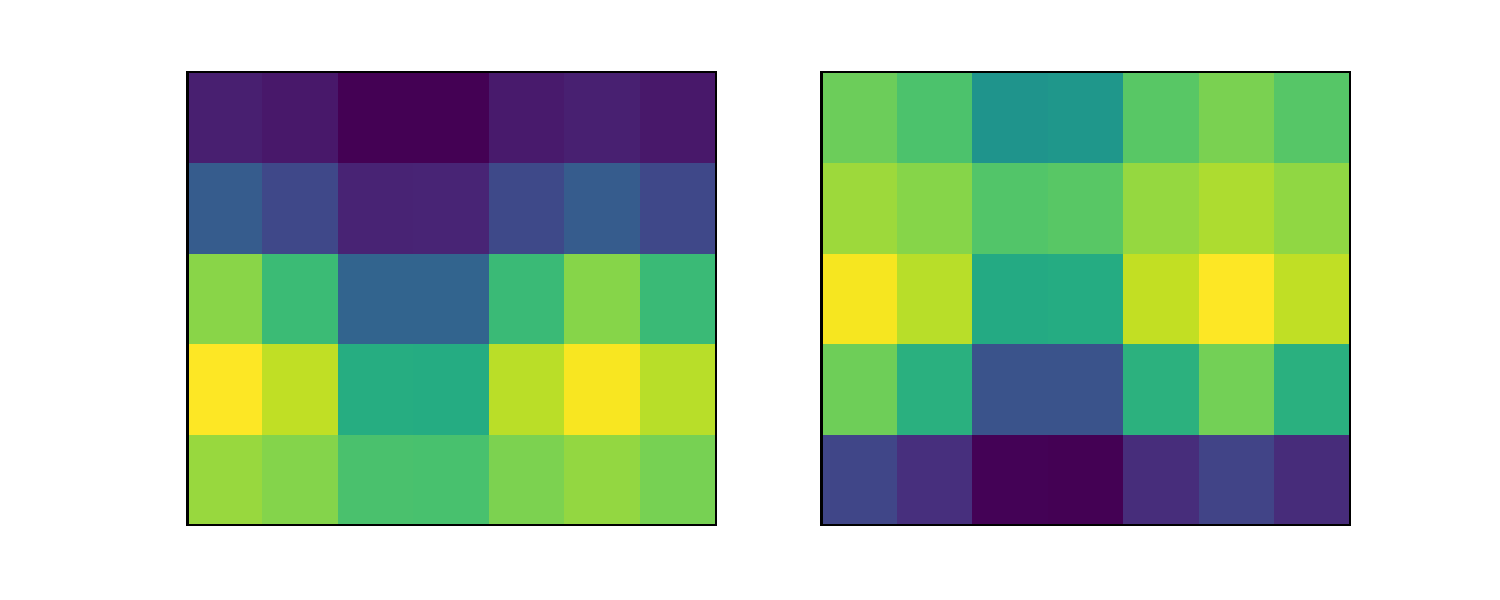
\includegraphics[width=.7\linewidth]{Figures/true_var_spatial}		
	
	\caption{Variance function at $t=25$ (left) and $t=45$ (right)} \label{fig:true_var_spatial}
\end{figure}

The left panel of \autoref{fig:true_fitted_var} shows the convergence of the two algorithms. Each iteration of the linearized algorithm takes about 0.01 seconds on average while each iteration of the consensus ADMM takes about 20 seconds. 


We estimated the linearized ADMM for all combinations of values of $\lambda_t$ and $\lambda_s$ from the sets $\lambda_t \in \{0,1,5,10,50,100\}$ and $\lambda_s \in \{0,0.05,0.1,0.2,0.3\}$. For each pair, we then compute the mean absolute error (MAE) between the estimated variance and the true variance at all locations and all time steps. For $\lambda_t=5$ and $\lambda_s=0.1$ MAE was minimized. The right panel of \autoref{fig:true_fitted_var} shows the true and the estimated standard deviation at location (0,0) using $\lambda_s=0.1$ and $\lambda_t=5$ (blue) and $\lambda_t=100$ (green). As we can see, larger than optimal value of $\lambda_t$ leads to estimated values which are ``too smooth". 

\begin{figure}[!h]
	\centering	
	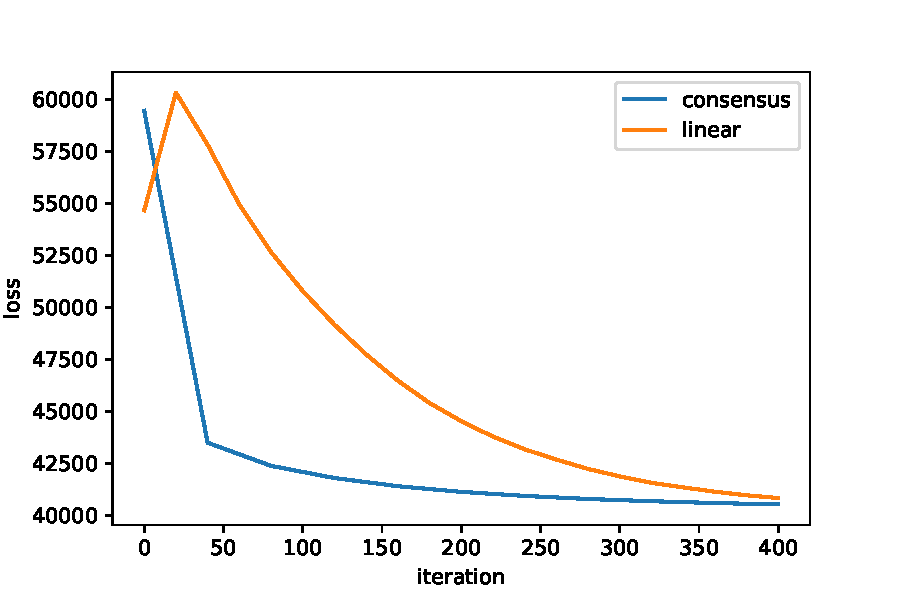
\includegraphics[width=.4\linewidth]{Figures/convergence}			
	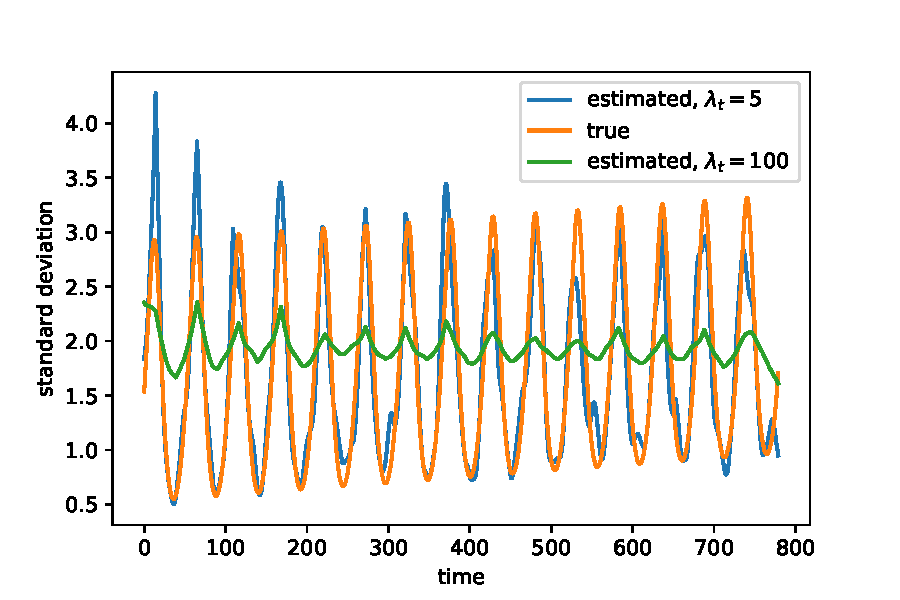
\includegraphics[width=.4\linewidth]{Figures/true_fitted_var}		
	\caption{Left: Convergence speed of linearized and consensus ADMM. Right: The true (orange) and estimated standard deviation function at the location (0,0). The estimated values are obtained using linearized ADMM with $\lambda_s=0.1$ and two values of $\lambda_t$: $\lambda_t=5$ (blue) and $\lambda_t=100$ (green).} \label{fig:true_fitted_var}
\end{figure}

\subsection{Data analysis}
As it was mentioned before, the algorithm proposed in \autoref{sec:consOpt} is appropriate only if we parallelize it over multiple machines and so we do not pursue it further here. All the results reported in this section are obtained using the linearize ADMM algorithm of \autoref{sec:linADMM}. We applied this algorithm on a subset of the ERA-40 dataset. The data is the 2 meter temperature measured daily at 12 p.m from August 31 of 1992 to 2002. To reduce the noise we first computed the weekly average of this data. To further reduce the size of the data, we will only analyze the data of the locations inside a rectangle extended from (\ang{58},\ang{226}) to (\ang{22},\ang{302}). This rectangle covers the united states. All the computations were performed on a machine with four 3.20GHz Intel i5-3470 cores.

\paragraph{Data Exploration}
The red curve in the left panel of \autoref{fig:bloom_estimatedSD} shows the estimated SD (which is $\exp(h_t/2)$) of the residuals of the time-series of Bloomington. To reduce the number of time-steps in this figure and in the remainder of the paper we work on the weekly averaged of the data. 

The curve of the estimated SD captures the periodic variations in the SD of the signal. Just by looking at this curve, it is hard to say if the SD is decreasing or increasing. Therefore, we compute the average of the estimated SD for each year. The estimated SD together with this annual average is shown in the middle panel of \autoref{fig:bloom_estimatedSD}. As it can be seen, the annual trend is not smooth. This is because in the optimization problem \eqref{eq:l1tf_var}, the smoothness of the annual trend is not encouraged. To remedy this, we add the following long horizon penalty to \eqref{eq:l1tf_var}:

\begin{equation}
\sum_{i=1}^{N_{year}-2} \Big\arrowvert \sum_{t=1}^{52} h_{t_1}-2h_{t_2}+h_{t_3}  \Big\arrowvert
\label{eq:lh_penalty}
\end{equation}

 where $t_1=52(i-1)+t$, $t_2=52i+t$ and $t_3=52(i+1)+t$. Also, $N_{year}$ is the number of years over which we are performing our analysis (here $N_{year}=10$). Since we are working on the weekly averaged data, each year corresponds to 52 observations. In the matrix form, the penalty \eqref{eq:lh_penalty} adds $N_{year}$ rows to the matrix $D$. The estimated SDs using this penalty matrix is shown in the right panel of \autoref{fig:bloom_estimatedSD}. The annual average of the estimated SDs shows a linear trend with a positive slope.

\begin{figure}[tb]
	\vskip 0.2in
	\begin{center}
		\centerline{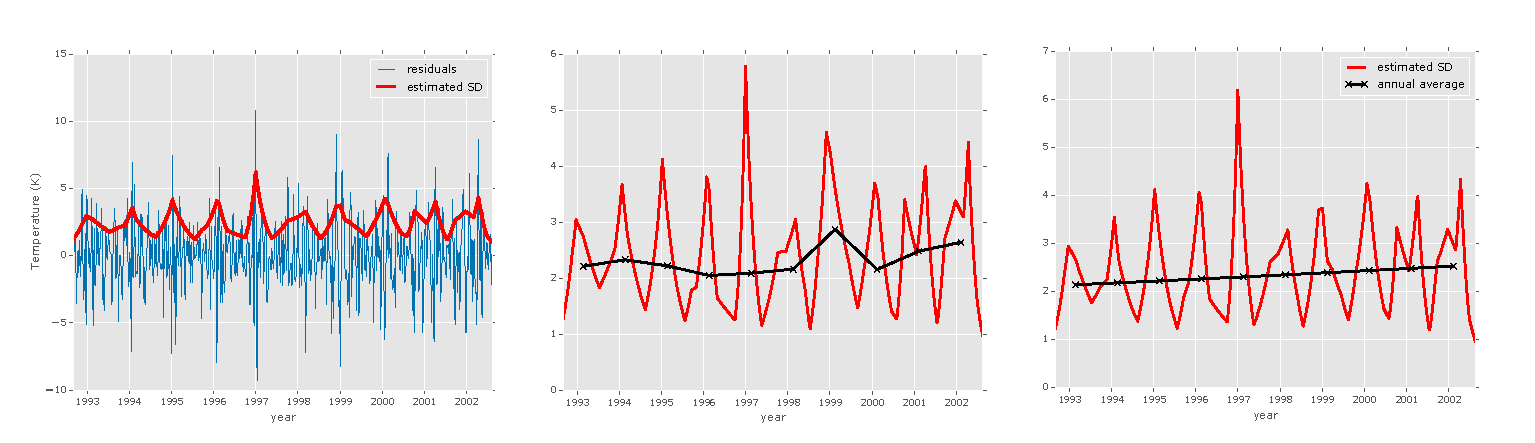
\includegraphics[width=\columnwidth]{Figures/bloom_estimatedSD}}
		\caption{Left: The residuals of the time-series of Bloomington (averaged weekly) and the estimated SD obtained from the method of \autoref{sec:l1tf_var} (red). Middle: the estimated SDs (red) and their annual average (black) without imposing the long horizon penalty. Right: the same as middle panel but here the long horizon penalty is imposed. See the text for more details.}
		\label{fig:bloom_estimatedSD}
	\end{center}
	\vskip -0.2in
\end{figure} 

%TODO: how to choose lambda? plot BIC as a function of lambda. 


This section is devoted to exploring some of the properties of the ERA-40 surface temperature data set. The goal here is to demonstrate some of the difficulties in modeling the trend in the temperature volatility and motivate our methodology for doing so.

% \autoref{fig:cities_ts} shows the time-series of the temperature of three cities: Bloomington (USA), San Diego (USA) and Manaus (Brazil). The time-series of Bloomington and San Diego show clear cyclic behavior. However, while it seems (qualitatively) that these cycles can be modeled by a sinusoidal function for Bloomington, the same is not true for San Diego. Also, the amplitude of the cycles changes from some years to others. The time-series of Manaus does not show any regular cyclic behavior. This demonstrates the first difficulty in analyzing the variance of this data: to analyze the variance, we first need to remove the cyclic terms from all time-series. However, there is a lot of variations in the cyclic behavior of the time-series of different locations. In addition, some of these cycles cannot be easily modeled by a parametric function \footnote{One might try to model the cycles by the summation of sinusoidal terms with different frequencies. However, for some time-series this may need many terms to be included in the summation to achieve a reasonable level of accuracy. In addition, this model cannot capture the non-stationarity in the cycles.}. To overcome these issues, we will use a non-parametric approach to remove the cyclic terms from the time-series and de-trend them. This approach, called \textit{$\ell_1$-trend filtering} is explained in the next section.

% \begin{figure}[tb]
% 	\vskip 0.2in
% 	\begin{center}
% 		\centerline{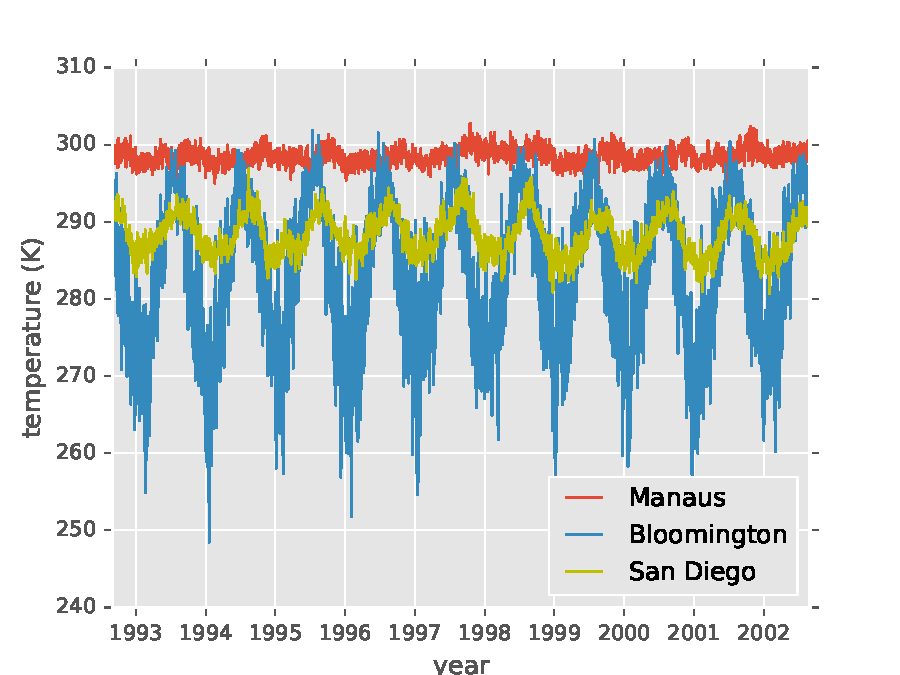
\includegraphics[width=\columnwidth]{Figures/cities_ts}}
% 		\caption{Time-series of the temperature (in Kelvin) of three cities.}
% 		\label{fig:cities_ts}
% 	\end{center}
% 	\vskip -0.2in
% \end{figure} 

The right panel of \autoref{fig:bloom_detrended} shows the time-series of the temperature of Bloomington, after removing the cyclic terms and de-trending using the method explained in the next section. The goal is to investigate the trend in the variance of this signal. This figure, reveals another issue toward this goal: the variance of this signal, shows cyclic behavior. Also, the cycles are not regular and their amplitude and frequency change. Even if one can describe the behavior of the variance of all the time-series using a single parametric model (for example a variant of the GARCH models \citep{bollerslev_generalized_1986}), it is not clear how the trend in the variance should be investigated in this framework. These observations motivate the need to develop a non-parametric framework for the problem at hand.

\begin{figure}[tb]
	\vskip 0.2in
	\begin{center}
		\centerline{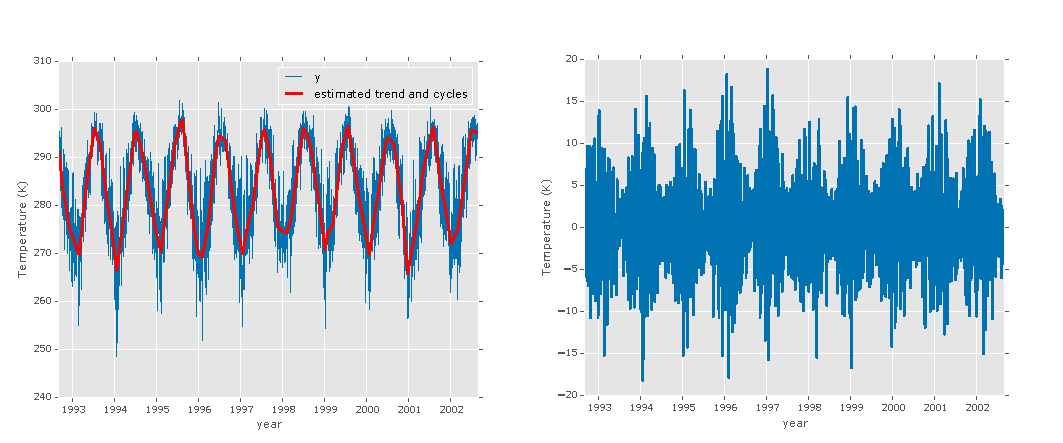
\includegraphics[width=\columnwidth]{Figures/bloom_trend_resid}}
		\caption{Left: Time-series of the temperature of Bloomington (blue) and the estimated trend and cycles obtained from the $\ell_1$-trend filtering (red). Right: the same time-series after removing the cyclic terms and de-trending using $\ell_1$-trend filtering.}
		\label{fig:bloom_detrended}
	\end{center}
	\vskip -0.2in
\end{figure} 


\paragraph{Convergence}

We used the following rule to determine when to stop the optimization: the optimization was stopped if the value of the loss did not improve by at least 0.1\% in 1000 trials. As we can see, the algorithm converged in about 2000 iterations. This took about 11 minutes. Our experiments showed that the convergence speed depends on the value of $\lambda_t$ and $\lambda_s$. Also, if we use the solution obtained for smaller values of these parameters as the initial value for the larger values (\textit{warm start}), the converges speed improves.


\paragraph{Model selection}
One common method for choosing the penalty parameters in the Lasso problems is to find the solution for a range of the values of these parameters and then choose the values which minimize a model selection criterion. However, such analyses needs the computation of the degrees of freedom (df). Several previous work have investigated the df in generalized lasso problems \citep{tibshirani_degrees_2012,hu_dual_2015,zeng_geometry_2017}. However, all these studies have considered the linear regression problem and, to the best of our knowledge, the problem of computing the df for generalized lasso with general objective function has not been considered yet.

Another approach is to choose the set of values which minimize an estimate of the expected prediction error obtained by k-fold cross-validation \citep{tibshirani_regression_1996} . Although this method is applicable for our problem, it needs k times more computation.

In this paper, we use a heuristic method for choosing $\lambda_t$ and $\lambda_s$: we compute the optimal solution for a range of values of these parameters and choose the values which minimize $\mathscr{L}(\lambda_t,\lambda_s)=-l(y|h)+ \sum \lVert D_{total}h \lVert$. This objective is a compromise between the negative log likelihood ($-l(y|h)$) and the complexity of the solution ($\sum \lVert D_{total}h \lVert$). For smoother solutions the value of $\sum \lVert D_{total}h \lVert$ will be smaller but with the cost of larger $-l(y|h)$.

We computed the optimal solution for all the combinations of the following sets of values: $\lambda_t \in \{1,5,10,20\} \, \, , \lambda_s \in \{0,.1,1,5,10\}$. The best combination based on a held out set was $\lambda_t=5$ and $\lambda_s=1$. All the analyses in the next section are performed on the solution for these values.


\paragraph{Analysis of trend of temperature volatility}

The top row of \autoref{fig:avg_change_estimatedSD} shows the detrended data, the estimated standard deviation and the yearly average of these estimates for two cities in the US. The estimated SD captures the periodic behavior in the variance of the time-series. In addition, the number of linear segments changes adaptively in each time window depending on how fast the variance is changing. 
The yearly average of the estimated SD captures the trend in the temperature volatility. For example, we can see that in Bloomington, there is a small positive trend. To determine how the volatility has changed in each location, we subtract the average of the estimated variance in 1992 from the average in the following years and compute their sum. The value of this change in the variance in each location is depicted in the right panel of \autoref{fig:avg_change_estimatedSD}. The left panel of this figure, shows the average estimated variance in each location.

\begin{figure}[tb]
	  \centering
          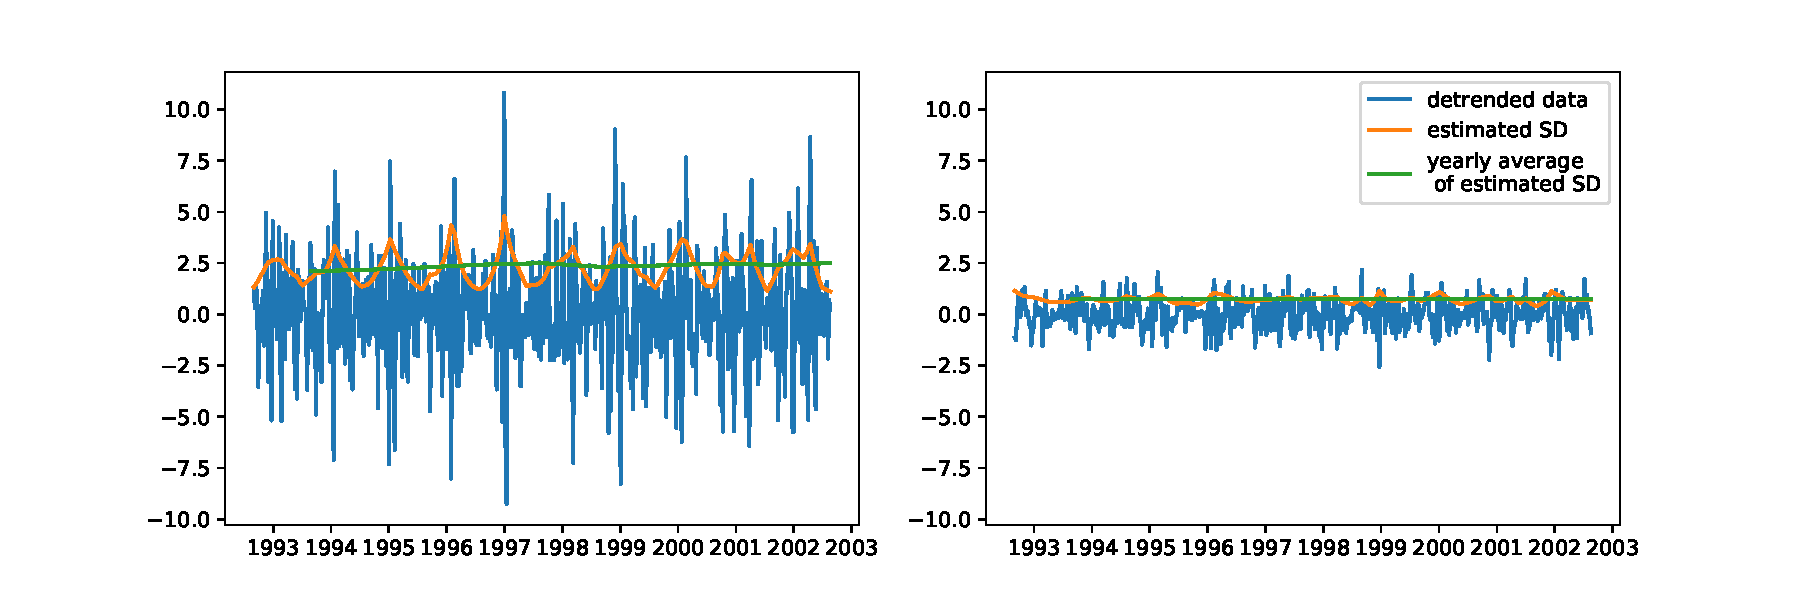
\includegraphics[width=.9\columnwidth]{Figures/estimatedSD}\\
	  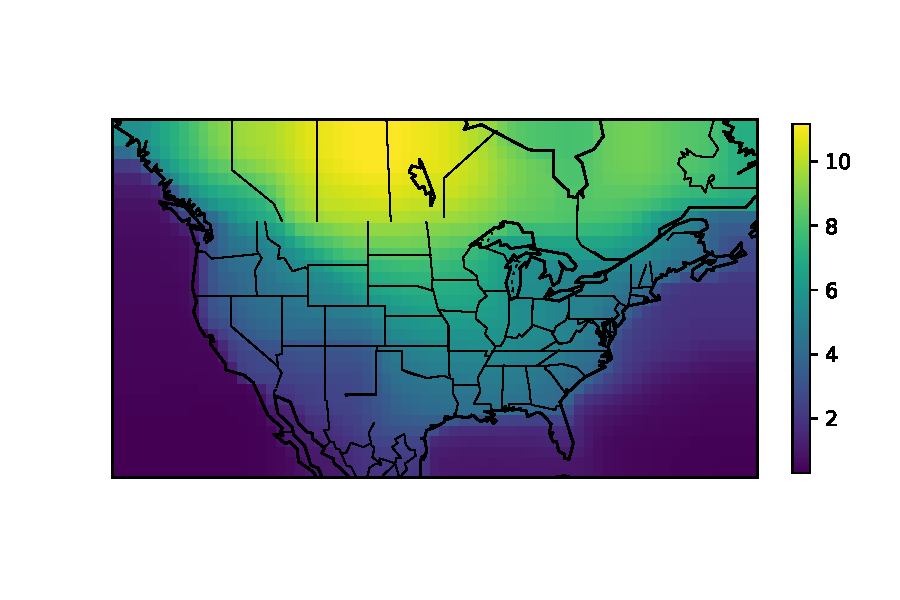
\includegraphics[width=.45\linewidth]{Figures/avg_estimatedVar}
	  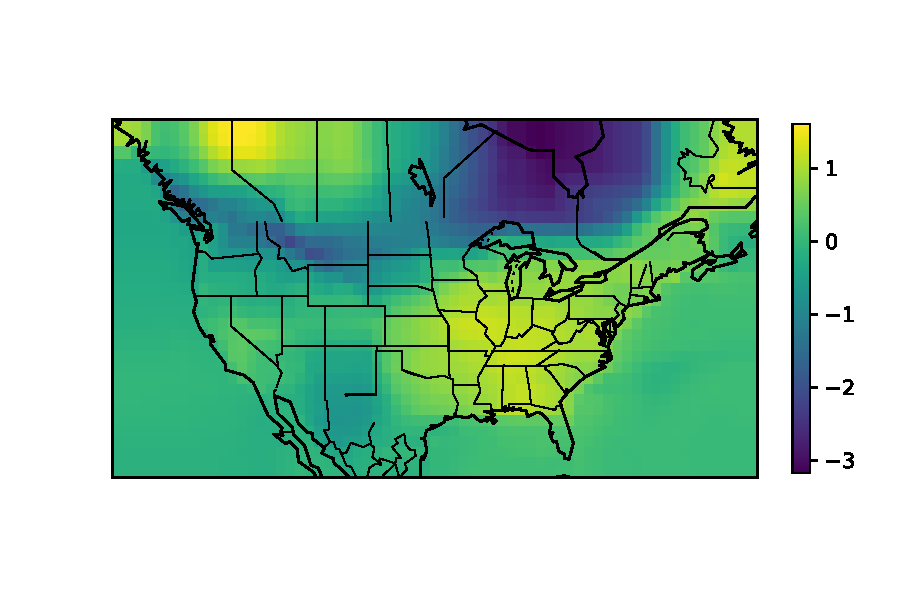
\includegraphics[width=.45\linewidth]{Figures/avg_change_estimatedVar}
	\caption{Top row: Detrended data and the estimated SD for Bloomington (left) and San Diego (right). Bottom: the average of the estimated variance over the US (left) and the change in the variance from 1992 to 2002 (right)}
	\label{fig:avg_change_estimatedSD}
\end{figure} 
It is interesting to note that the trend in volatility is almost zero over the oceans. The most positive trend can be observed in the south-east and the most negative trend has happened in the north-east. 
 

\section{Discussion}
In this paper, we proposed a new method for estimating the variance of spatio-temporal data. The main idea is to cast this problem as a constrained optimization problem where the constraints enforce smooth changes in the variance for neighboring points in time and space. In particular, the solution is piecewise linear in time and piecewise constant in space. The resulting optimization is in the form of a generalized LASSO problem with high-dimension, and so applying the PDIP method directly is infeasible. We therefore developed two ADMM-based algorithms to solve this problem: the consensus ADMM and linearized ADMM.

The consensus ADMM algorithm converges in few hundreds of iterations but each iteration takes much longer than the linearized ADMM algorithm. The appealing feature of the consensus ADMM algorithm is that if it is parallelized on enough number of machines the computation time per iteration remains constant as the problem size increases. The linearized ADMM algorithm, on the other hand converges in few thousands of iterations but each iteration is performed in split second. However, since the algorithm converges in many iterations it is not very appropriate for parallelization. The reason is that after each iteration the solution computed in each machine should be broadcast to the master machine and this operation takes some time which depends on the speed of the network connecting the slave machines to the master. A direction for future research would be to combine these two algorithms in the following way: the problem should be split into the sub-problems (as in the consensus ADMM) but each sub-problem can be solved using linearized ADMM.

We applied the linearized ADMM algorithm to the surface temperature data on a grid over the united states, for years 1992-2002. The results showed that in many locations the variance of the temperature has increased about 1 unit in 10 years.

The goal of this paper, however, is not to make any conclusions about the trend in the variance because we solved the problem only for a grid over the united states and for 10 years of the data. A thorough analysis, needs the full solution over the globe and for a longer time period. The goal of the paper, was to propose the idea of estimating the trend in variance of spatio-temporal signals using generalized lasso and to investigate the algorithms for solving the resulting optimization problem.


\bibliographystyle{abbrvnat}
\small
\bibliography{nips-references}


\end{document} 

